%%%%%%%%%%%%%%%%%%%%%%%%%%%%%%%%
% Settings
%%%%%%%%%%%%%%%%%%%%%%%%%%%%%%%%

\usetikzlibrary{arrows.meta}




%%%%%%%%%%%%%%%%%%%%%%%%%%%%%%%%%%
\definecolor{blueA}{RGB}{54, 75, 154}
\definecolor{blueB}{RGB}{74, 123, 183}
\definecolor{blueC}{RGB}{209, 229, 240}

\colorlet{newMessageFill}{blueC}
\colorlet{newMessageDraw}{blueB}
\colorlet{messageFill}{white}
\colorlet{messageDraw}{black}
\colorlet{moduleFrame}{black!80!white}
\colorlet{moduleFill}{black!30!white}
%\colorlet{moduleFill}{blueB}
\colorlet{moduleContentFill}{black!10!white}

\tikzset{thickArrow/.style={
		-{Latex[length=1.5mm,width=1.5mm]},
%		-{Latex[length=1mm,width=2mm]},
		thick,
		rounded corners=1ex
	}
}
\tikzset{newThickArrow/.style={
		thickArrow,
		very thick,
		rounded corners=1ex,
		newMessageDraw,
	}
}

\tikzset{module/.style={
		rounded corners=1ex,
		draw=moduleFrame,
		fill=moduleFill,
		inner sep=0
	}
}
\tikzset{moduleContent/.style={
		rounded corners=1ex,
		draw=moduleFrame,
		fill=moduleContentFill,
		inner sep=0
	}
}

\tikzset{message/.style={
		rectangle,
		rounded corners=1ex,
		minimum width=19ex,
		minimum height=3.5ex,
		draw=messageDraw,
		fill=messageFill
	}
}
\tikzset{newMessage/.style={
		rectangle,
		rounded corners=1ex,
		minimum width=19ex,
		minimum height=3.5ex,
		thick,
		draw=newMessageDraw,
		fill=newMessageFill
	}
}


\newcommand{\va}{\bm{a}}
\newcommand{\vz}{\bm{z}}
\newcommand{\vb}{\bm{b}}
\newcommand{\vtheta}{\bm{\theta}}
\newcommand{\jac}{\mathrm{J}}
\newcommand{\mS}{\bm{S}}

\newcommand{\mynablasub}[1]{\nabla\raise-0.5ex\hbox{\text{\tiny$\kern -0.5em  #1$}}\kern 0.1em}
\newcommand{\myjacsub}[1]{\jac\raise-0.25ex\hbox{\text{\tiny$\kern -0.0em  #1$}}\kern 0.1em}


\small
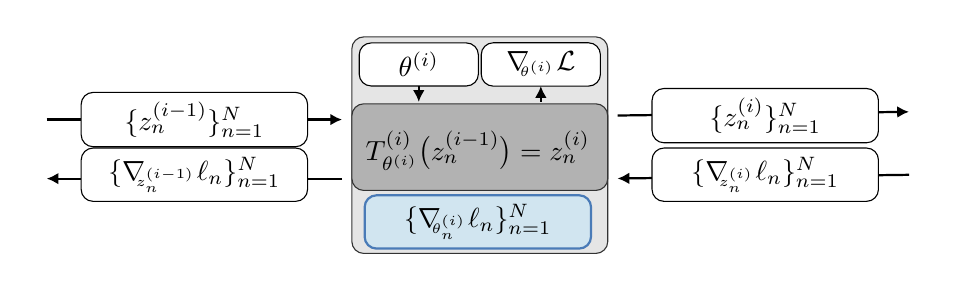
\begin{tikzpicture}
\node (v1) at (0.75,1) {};
\node (v2) at (-2.5,2.95) {};
\node (v3) at (-2.5,2.1) {};
\node (v12) at (0.75,0.2) {};

\draw[moduleContent] (v2) rectangle (v12);

\node (v4) at (4.7,2) {};
\node (v6) at (4.7,1.2) {};

\node (v5) at (0.75,1.95) {};
\node (v7) at (0.75,1.15) {};
\draw[thickArrow] (v5) edge (v4);
\draw[thickArrow] (v6) edge (v7);
\node (v10) at (-2.5,1.9) {};
\node (v12) at (-2.5,1.15) {};

\node (v11) at (-6.5,1.9) {};
\node (v13) at (-6.5,1.15) {};

\draw[thickArrow] (v11) edge (v10);
\draw[thickArrow]  (v12) edge (v13);

\node[message] at (-4.5,1.9) {$\{\vz^{(i-1)}_n\}_{n=1}^N$};
\node[message] at (2.75,1.95) {$\{\vz^{(i)}_n\}_{n=1}^N$};
\node[message] at (-4.5,1.2) {$\{ \mynablasub{\vz_n^{(i-1)}} \ell_n \}_{n=1}^N$};
\node[message] at (2.75,1.2) {$\{\mynablasub{\vz^{(i)}_n} \ell_n\}_{n=1}^N$};

\node[newMessage] at (-0.9,0.6) {$\{\mynablasub{\vtheta^{(i)}_n} \ell_n\}_{n=1}^N$};

% Inner messages

\node (v18) at (-0.1,2) {};
\node (v19) at (-0.1,2.45) {};
\draw[thickArrow] (v18) edge (v19);
\node[message,minimum width=10ex] at (-0.1,2.6) {$\mynablasub{\vtheta^{(i)}} \mathcal{L}$};

\node (v16) at (-1.65,2.7) {};
\node (v17) at (-1.65,2) {};
\draw[thickArrow] (v16) edge (v17);
\node[message,minimum width=10ex] at (-1.65,2.6) {$\vtheta^{(i)}$};

\draw[module] (v3) rectangle (v1) {};
\node at (-0.9,1.5) {$T^{(i)}_{\vtheta^{(i)}}\big(\vz^{(i-1)}_n\big) = \vz^{(i)}_n$};

\end{tikzpicture}